The final stage is the classification stage. The inputs to this stage are the max-pooled masked images and feature vectors described in section \ref{preprocessing}. However, instead of using this as a direct input for classification, we try to reduce this data further as our objective is to reduce computational complexity and get a good runtime.

Principal component analysis (PCA) is a data transformation technique used to reduce the dimensionality of high-dimensional data into a low-dimensional subspace while maintaining most of the variance \cite{b5_1,b5_2}. The use of PCA to reduce the dimensionality of the inputs is a possibility if it does not result in a drastic drop in accuracy. The reduced data can be used as the input for classification as illustrated in Fig. \ref{fig:pca}.

We investigate using an ensemble classifier to compare accuracy. The ensemble method is a powerful technique that combines multiple models into a single predictive model. This often makes it more accurate and reliable than its individual components \cite{b5_3}. The classifier we propose is a decision tree classifier wrapped in a bagging based ensemble model. The bagging method selects a random subset of the dataset with replacements for training each model and uses a voting scheme to make a final prediction \cite{b5_4}. One of the more prominent examples of a bagged decision tree model is the random forest classifier \cite{b5_5}.

\begin{figure}[tp]
	\centerline{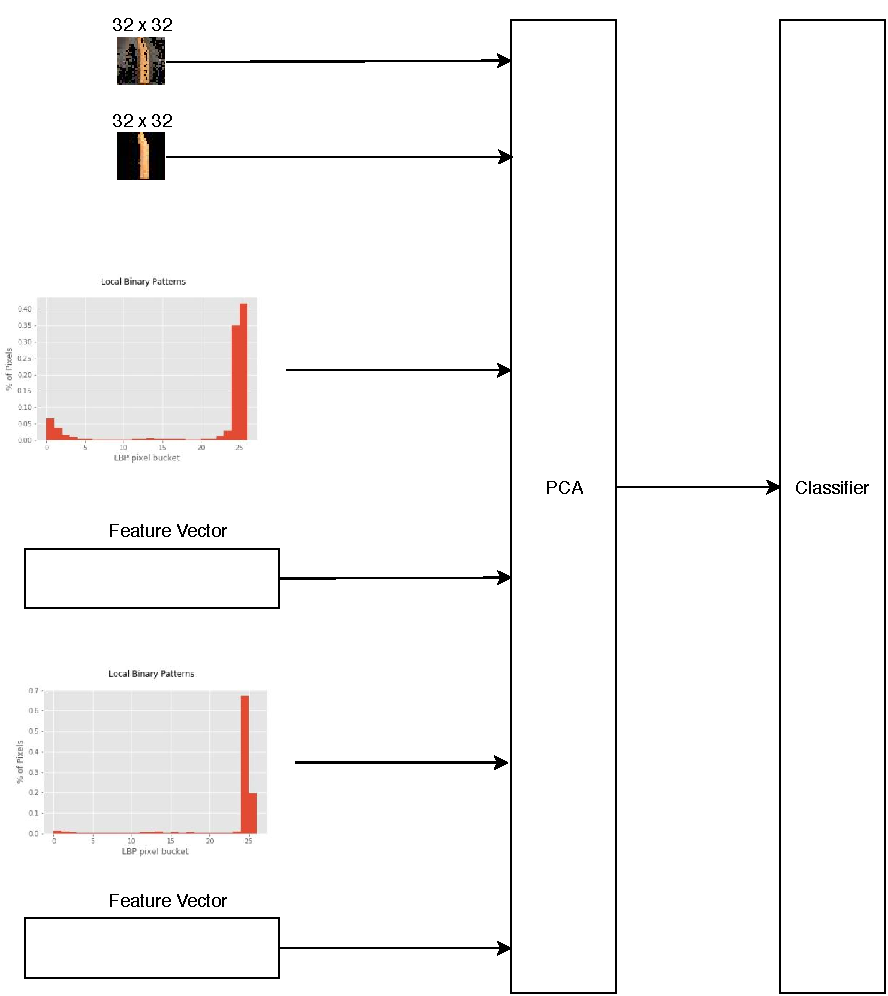
\includegraphics[scale=0.5]{./img/pca.pdf}}
	\caption{The steps to transform the input before classification.}
	\label{fig:pca}
\end{figure}